% Drawing 154/07-6 -- folder 154, batch 07, archive page 128 (PDF page 129).
% Transcription: dessins en couleur, sans texte : trois graphes superposés, bleu, vert et orange, autour d'un sommet bleu central, avec six petits carrés bruns aux sommets de l'hexagone orange ; une étoile bleue à huit branches ; un sommet bleu entouré d'un cercle orange hachuré ; un graphe vert en tirets ; un hexagone vert portant des triangles orange à ses sommets, traversé de rayons bleus
% Kind: blue map, green dual and orange medial graph round a blue vertex; blue star; vertex in a hatched orange ellipse; dashed green graph; green pentagon with orange vertex links. Method 2 (redrawn from the facsimile). Status: partial.
% Notes: Colour drawings without text, over a job log (not reproduced), redrawn from the 400 dpi crop. First figure: three superposed graphs, read as a blue map, its green dual and the orange medial graph. Blue: ten vertices (the central one of degree eight), every edge drawn through the point where its dual green edge crosses it; green: eight vertices and seven free ends, each green edge a broken line through that crossing point; orange: twenty-six segments, each joining two such crossing points, so that every orange segment, green edge and blue edge meets the others exactly at these points. The six brown squares sit on the six spokes from the central blue vertex at their crossings with the green edges (the orange hexagon), with the four small brown dots on its sides. Near the centre, three points (between the centre and the squares) where a blue half-edge, a green half-edge and two orange segments all stop short: drawn stopping at the same small gap (0.45 mm) from a common point, as on the page. Pencil: the lens from a green vertex to the centre, the line from the lower left green vertex to the centre and the hatched triangle it bounds with the green edge and the blue spoke (hatching bounded exactly by these three strands); faint pencil ovals under the bottom squares left out. Second figure: a blue star of seven branches (four ending in dots) and a short doubled stroke on the upper left branch. Third: a blue vertex with eight rays (four ending in blue dots, four in small brown dots, four brown ticks), an orange ellipse crossed by them, its pencil hatching drawn as parallel lines clipped to the ellipse; an orange U-shaped arc crossed by one ray, with four pencil hatch strokes. Fourth: the dashed green graph (five vertices, solid and dashed edges) with the dark pencil stroke and the faint pencil lines below it. Fifth: a green pentagon (not a hexagon) with a blue vertex inside joined by five rays crossing its five sides, plus a dashed blue ray towards the upper right corner; the orange pieces at the corners are links of the green vertices, each orange corner placed exactly on the green edges it joins (a chord at three corners, a quadrilateral with a dashed side at the lower left, a pentagon at the upper right). Still to check: the cut points near the centre of the first figure (drawn as gaps). Redrawn 2026-11-09 (issue 128): to check again.
% Coordinates: 1 unit = 1 mm = 1/100 of the crop width (bbox in page fractions: [0.148, 0.101, 0.9, 0.496]).
% Redrawn by Claude (claude-opus-5-5), issue #73, 2026-11-07; not checked by a human; not compiled (no TeX in the session).
% Revised by Claude (claude-opus-5-5) 2026-11-09 (issue #128) after Michel's check: vertices snapped to exact intersections (drawn points on their lines, meeting ends on the stroke they meet, near-concurrent lines through one computed point, curve ends on their rim); labels at \small as in folder 80 batch 3. Status: partial.
% Redrawn by Claude (claude-opus-5-5) 2026-11-09 (issue #128, further pass): all five figures redrawn from the 400 dpi crop: first figure as blue map, green dual and orange medial graph meeting exactly at the computed blue/green crossing points. Not compiled. Status: partial.
% Rights: reproduces part of the work -- behind RENDER_TRANSCRIPTS, never published by itself.
\documentclass[tikz,border=3pt]{standalone}
\usepackage{amsmath,amssymb}
\usetikzlibrary{patterns,arrows.meta}
\tikzset{Or/.style={orange!90!black}, Ye/.style={yellow!80!orange}, Lg/.style={green!60!black!70}, Dg/.style={green!45!black}, Br/.style={brown!80!black}, Rd/.style={red!85!black}, Bl/.style={blue!70!black}, Gy/.style={black!40}, pencil/.style={black!45}, struck/.style={black!35}, mark/.style={circle,draw,inner sep=1.3pt}, pt/.style={circle,fill,inner sep=0.9pt}, opt/.style={circle,draw,fill=white,inner sep=1.1pt}}
\colorlet{Or}{orange!90!black}\colorlet{Ye}{yellow!80!orange}\colorlet{Lg}{green!60!black!70}\colorlet{Dg}{green!45!black}\colorlet{Br}{brown!80!black}\colorlet{Rd}{red!85!black}\colorlet{Bl}{blue!70!black}\colorlet{Gy}{black!40}
\begin{document}
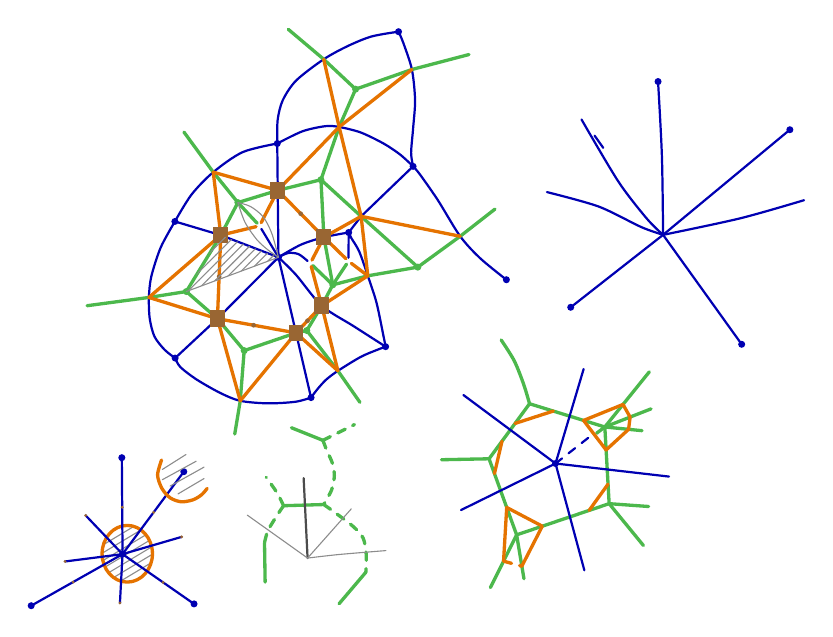
\begin{tikzpicture}[x=1mm,y=1mm,line cap=round,line join=round,font=\scriptsize]
\draw[Bl,thick] plot[smooth, tension=0.5] coordinates {(47.6,-1.2) (44.2,-1.8) (41.2,-3) (38.1,-4.7) (34.6,-7.4) (32.9,-9.9) (32.25,-12.4) (32.2,-15.4)};
\draw[Bl,thick] plot[smooth, tension=0.5] coordinates {(47.6,-1.2) (48.2,-2.6) (49.3,-6) (49.7,-9.9) (49.45,-13.5) (49.2,-16.6) (49.45,-18.3)};
\draw[Bl,thick] plot[smooth, tension=0.5] coordinates {(32.2,-15.4) (35.4,-13.85) (38.3,-13.2) (40.06,-13.3) (42.8,-14) (45.7,-15.4) (47.8,-16.8) (49.45,-18.3)};
\draw[Bl,thick] plot[smooth, tension=0.5] coordinates {(32.2,-15.4) (27.8,-16.5) (24.07,-19.04) (21.3,-21.9) (19.2,-25.3)};
\draw[Bl,thick] plot[smooth, tension=0.5] coordinates {(19.2,-25.3) (17.4,-28.6) (16.2,-32.3) (15.9,-34.95) (16,-37.6) (16.6,-39.9) (17.9,-41.6) (19.23,-42.65)};
\draw[Bl,thick] plot[smooth, tension=0.5] coordinates {(19.23,-42.65) (19.9,-43.8) (22,-45.4) (25,-47.1) (27.5,-48.08) (31,-48.4) (34.5,-48.2) (36.49,-47.67)};
\draw[Bl,thick] plot[smooth, tension=0.5] coordinates {(36.49,-47.67) (37.3,-46.6) (38.4,-45.4) (39.9,-44.27) (42.8,-42.5) (44.9,-41.6) (45.96,-41.2)};
\draw[Bl,thick] plot[smooth, tension=0.5] coordinates {(45.96,-41.2) (45.7,-39.9) (44.8,-35.6) (43.7,-32.2) (42.6,-29.1) (41.6,-27.4) (41.27,-26.7)};
\draw[Bl,thick] (49.45,-18.3) -- (42.85,-24.65) -- (41.27,-26.7);
\draw[Bl,thick] plot[smooth, tension=0.5] coordinates {(49.45,-18.3) (50.3,-19.3) (52.6,-22.6) (55.43,-27.18) (58,-30) (61.3,-32.7)};
\draw[Bl,thick] (32.2,-15.4) -- (32.26,-21.35) -- (32.35,-29.85);
\draw[Bl,thick] (19.2,-25.3) -- (25.03,-27.04) -- (32.35,-29.85);
\draw[Bl,thick] (19.23,-42.65) -- (24.6,-37.65) -- (32.35,-29.85);
\draw[Bl,thick] (32.35,-29.85) -- (34.58,-39.45) -- (36.49,-47.67);
\draw[Bl,thick] plot[smooth, tension=0.5] coordinates {(32.35,-29.85) (34.6,-32.1) (37.85,-36) (41.9,-38.6) (45.96,-41.2)};
\draw[Bl,thick] plot[smooth, tension=0.5] coordinates {(32.35,-29.85) (35.2,-28.25) (38.12,-27.3) (41.27,-26.7)};
\draw[Bl,thick] (32.35,-29.85) -- (30.18,-26.24);
\draw[Bl,thick] plot[smooth, tension=0.5] coordinates {(32.35,-29.85) (33.6,-29.3) (34.9,-29.45) (36.05,-30.32)};
\draw[Bl,thick] (41.27,-26.7) -- (41.25,-29.9);
\node[pt,Bl] at (32.35,-29.85) {};
\node[pt,Bl] at (47.6,-1.2) {};
\node[pt,Bl] at (32.2,-15.4) {};
\node[pt,Bl] at (49.45,-18.3) {};
\node[pt,Bl] at (19.2,-25.3) {};
\node[pt,Bl] at (41.27,-26.7) {};
\node[pt,Bl] at (61.3,-32.7) {};
\node[pt,Bl] at (19.23,-42.65) {};
\node[pt,Bl] at (45.96,-41.2) {};
\node[pt,Bl] at (36.49,-47.67) {};
\draw[Lg,very thick] (33.6,-0.9) -- (38.1,-4.7) -- (42.15,-8.5);
\draw[Lg,very thick] (42.15,-8.5) -- (49.3,-6) -- (56.55,-4.1);
\draw[Lg,very thick] (42.15,-8.5) -- (40.06,-13.3) -- (37.75,-20);
\draw[Lg,very thick] (37.75,-20) -- (32.26,-21.35) -- (27.2,-22.9);
\draw[Lg,very thick] (37.75,-20) -- (42.85,-24.65) -- (50.05,-31.1);
\draw[Lg,very thick] (37.75,-20) -- (38.12,-27.3) -- (39.25,-33.35);
\draw[Lg,very thick] (27.2,-22.9) -- (24.07,-19.04) -- (20.35,-13.95);
\draw[Lg,very thick] (27.2,-22.9) -- (25.03,-27.04) -- (20.65,-34.2);
\draw[Lg,very thick] (20.65,-34.2) -- (15.9,-34.95) -- (8.05,-36);
\draw[Lg,very thick] (20.65,-34.2) -- (24.6,-37.65) -- (28,-41.7);
\draw[Lg,very thick] (28,-41.7) -- (34.58,-39.45) -- (35.95,-39.15);
\draw[Lg,very thick] (28,-41.7) -- (27.5,-48.08) -- (26.8,-52.3);
\draw[Lg,very thick] (35.95,-39.15) -- (37.85,-36) -- (39.25,-33.35);
\draw[Lg,very thick] (35.95,-39.15) -- (39.9,-44.27) -- (42.7,-48.27);
\draw[Lg,very thick] (39.25,-33.35) -- (43.7,-32.2) -- (50.05,-31.1);
\draw[Lg,very thick] (50.05,-31.1) -- (55.43,-27.18) -- (59.85,-23.73);
\draw[Lg,very thick] (27.2,-22.9) -- (29.64,-25.52);
\draw[Lg,very thick] (39.25,-33.35) -- (41,-30.72);
\draw[Lg,very thick] (39.25,-33.35) -- (36.72,-30.91);
\node[pt,Lg] at (37.75,-20) {};
\node[pt,Lg] at (27.2,-22.9) {};
\node[pt,Lg] at (42.15,-8.5) {};
\node[pt,Lg] at (20.65,-34.2) {};
\node[pt,Lg] at (50.05,-31.1) {};
\node[pt,Lg] at (39.25,-33.35) {};
\node[pt,Lg] at (28,-41.7) {};
\node[pt,Lg] at (35.95,-39.15) {};
\draw[Or,very thick] (32.26,-21.35) -- (40.06,-13.3);
\draw[Or,very thick] (32.26,-21.35) -- (24.07,-19.04);
\draw[Or,very thick] (32.26,-21.35) -- (38.12,-27.3);
\draw[Or,very thick] (25.03,-27.04) -- (24.07,-19.04);
\draw[Or,very thick] (25.03,-27.04) -- (15.9,-34.95);
\draw[Or,very thick] (25.03,-27.04) -- (24.6,-37.65);
\draw[Or,very thick] (24.6,-37.65) -- (15.9,-34.95);
\draw[Or,very thick] (24.6,-37.65) -- (34.58,-39.45);
\draw[Or,very thick] (24.6,-37.65) -- (27.5,-48.08);
\draw[Or,very thick] (34.58,-39.45) -- (27.5,-48.08);
\draw[Or,very thick] (34.58,-39.45) -- (37.85,-36);
\draw[Or,very thick] (34.58,-39.45) -- (39.9,-44.27);
\draw[Or,very thick] (37.85,-36) -- (43.7,-32.2);
\draw[Or,very thick] (37.85,-36) -- (39.9,-44.27);
\draw[Or,very thick] (38.12,-27.3) -- (42.85,-24.65);
\draw[Or,very thick] (40.06,-13.3) -- (38.1,-4.7);
\draw[Or,very thick] (40.06,-13.3) -- (49.3,-6);
\draw[Or,very thick] (40.06,-13.3) -- (42.85,-24.65);
\draw[Or,very thick] (42.85,-24.65) -- (55.43,-27.18);
\draw[Or,very thick] (42.85,-24.65) -- (43.7,-32.2);
\draw[Or,very thick] (32.26,-21.35) -- (30.16,-25.45);
\draw[Or,very thick] (25.03,-27.04) -- (29.51,-25.96);
\draw[Or,very thick] (38.12,-27.3) -- (40.93,-30.04);
\draw[Or,very thick] (43.7,-32.2) -- (41.61,-30.62);
\draw[Or,very thick] (38.12,-27.3) -- (36.61,-30.2);
\draw[Or,very thick] (37.85,-36) -- (36.52,-31.03);
\fill[Br] (35.18,-24.32) circle[radius=0.3];
\fill[Br] (24.82,-32.31) circle[radius=0.3];
\fill[Br] (29.2,-38.48) circle[radius=0.3];
\fill[Br] (36.04,-37.91) circle[radius=0.3];
\fill[Br] (31.31,-22.4) rectangle (33.21,-20.3);
\fill[Br] (24.08,-28.09) rectangle (25.98,-25.99);
\fill[Br] (23.65,-38.7) rectangle (25.55,-36.6);
\fill[Br] (33.63,-40.5) rectangle (35.53,-38.4);
\fill[Br] (36.9,-37.05) rectangle (38.8,-34.95);
\fill[Br] (37.17,-28.35) rectangle (39.07,-26.25);
\draw[pencil] plot[smooth, tension=0.5] coordinates {(27.2,-22.9) (28.1,-25.4) (29.6,-27.6) (31,-28.9) (32.35,-29.85)};
\draw[pencil] plot[smooth, tension=0.5] coordinates {(27.2,-22.9) (28.8,-23.4) (30.4,-24.7) (31.5,-26.8) (32.35,-29.85)};
\draw[pencil] (20.65,-34.2) -- (32.35,-29.85);
\fill[pattern=north east lines,pattern color=black!45] (20.65,-34.2) -- (25.03,-27.04) -- (32.35,-29.85) -- cycle;
\draw[Bl,thick] plot[smooth, tension=0.5] coordinates {(81.2,-27) (81.05,-17) (80.56,-7.53)};
\node[pt,Bl] at (80.56,-7.53) {};
\draw[Bl,thick] plot[smooth, tension=0.5] coordinates {(81.2,-27) (79.1,-24.9) (75.5,-20.2) (70.84,-12.35)};
\draw[Bl,thick] (72.5,-14.4) -- (73.6,-15.95);
\draw[Bl,thick] plot[smooth, tension=0.5] coordinates {(81.2,-27) (78.4,-26) (73,-23.4) (66.45,-21.57)};
\draw[Bl,thick] (81.2,-27) -- (69.47,-36.2);
\node[pt,Bl] at (69.47,-36.2) {};
\draw[Bl,thick] (81.2,-27) -- (91.18,-40.9);
\node[pt,Bl] at (91.18,-40.9) {};
\draw[Bl,thick] plot[smooth, tension=0.5] coordinates {(81.2,-27) (91,-24.9) (99.1,-22.6)};
\draw[Bl,thick] (81.2,-27) -- (97.3,-13.65);
\node[pt,Bl] at (97.3,-13.65) {};
\begin{scope}\clip (13.15,-67.5) ellipse[x radius=3.2, y radius=3.6];
\draw[pencil] (8.15,-64.55) -- (18.15,-58.55);
\draw[pencil] (8.15,-65.54) -- (18.15,-59.54);
\draw[pencil] (8.15,-66.54) -- (18.15,-60.54);
\draw[pencil] (8.15,-67.53) -- (18.15,-61.53);
\draw[pencil] (8.15,-68.52) -- (18.15,-62.52);
\draw[pencil] (8.15,-69.51) -- (18.15,-63.51);
\draw[pencil] (8.15,-70.5) -- (18.15,-64.5);
\draw[pencil] (8.15,-71.49) -- (18.15,-65.49);
\draw[pencil] (8.15,-72.48) -- (18.15,-66.48);
\draw[pencil] (8.15,-73.47) -- (18.15,-67.47);
\draw[pencil] (8.15,-74.46) -- (18.15,-68.46);
\draw[pencil] (8.15,-75.46) -- (18.15,-69.46);
\draw[pencil] (8.15,-76.45) -- (18.15,-70.45);
\end{scope}
\draw[Or,very thick] (13.15,-67.5) ellipse[x radius=3.2, y radius=3.6];
\draw[Bl,thick] (12.55,-67.55) -- (12.46,-55.3);
\node[pt,Bl] at (12.46,-55.3) {};
\draw[Bl,thick] (12.55,-67.55) -- (12.22,-73.75);
\fill[Br] (12.22,-73.75) circle[radius=0.2];
\draw[Bl,thick] (12.55,-67.55) -- (7.87,-62.64);
\fill[Br] (7.87,-62.64) circle[radius=0.2];
\draw[Bl,thick] (12.55,-67.55) -- (5.25,-68.48);
\fill[Br] (5.25,-68.48) circle[radius=0.2];
\draw[Bl,thick] (12.55,-67.55) -- (0.95,-74.1);
\node[pt,Bl] at (0.95,-74.1) {};
\draw[Bl,thick] (12.55,-67.55) -- (21.63,-73.87);
\node[pt,Bl] at (21.63,-73.87) {};
\draw[Bl,thick] (12.55,-67.55) -- (20.05,-65.36);
\fill[Br] (20.05,-65.36) circle[radius=0.2];
\draw[Bl,thick] (12.55,-67.55) -- (20.33,-57.08);
\node[pt,Bl] at (20.33,-57.08) {};
\fill[Br] (12.51,-61.6) circle[radius=0.2];
\fill[Br] (6.28,-71.09) circle[radius=0.2];
\fill[Br] (17.7,-71.14) circle[radius=0.2];
\fill[Br] (16.5,-62.24) circle[radius=0.2];
\node[pt,Bl] at (12.55,-67.55) {};
\draw[Or,very thick] plot[smooth, tension=0.5] coordinates {(17.5,-55.6) (17,-57.5) (17.55,-59.2) (18.6,-60.4) (20,-60.9) (21.5,-60.65) (22.6,-60) (23.3,-59.2)};
\draw[pencil] (17.6,-56.8) -- (20.6,-54.9);
\draw[pencil] (17.6,-58.1) -- (21.9,-55.75);
\draw[pencil] (18.6,-58.9) -- (22.9,-56.5);
\draw[pencil] (19.6,-59.9) -- (22.9,-57.95);
\draw[Lg,very thick] (38,-53.1) -- (34,-51.5);
\draw[Lg,very thick,dashed] (38,-53.1) -- (42,-51.1);
\draw[Lg,very thick,dashed] plot[smooth, tension=0.5] coordinates {(38,-53.1) (38.5,-54.4) (39.2,-56) (39.45,-57.6) (39.1,-59.4) (38.1,-61.25)};
\draw[Lg,very thick] (38.1,-61.25) -- (33,-61.4);
\draw[Lg,very thick,dashed] plot[smooth, tension=0.5] coordinates {(33,-61.4) (32.2,-59.8) (30.8,-57.8)};
\draw[Lg,very thick,dashed] plot[smooth, tension=0.5] coordinates {(33,-61.4) (32,-62.9) (31,-64.6) (30.58,-66.1)};
\draw[Lg,very thick] (30.58,-66.1) -- (30.66,-71.1);
\draw[Lg,very thick,dashed] plot[smooth, tension=0.5] coordinates {(38.1,-61.25) (39.3,-62.1) (41.8,-64) (43.1,-65.5) (43.5,-67.6) (43.45,-69.85)};
\draw[Lg,very thick] (43.45,-69.85) -- (40.05,-73.85);
\draw[black!70,thick] (35.55,-57.9) -- (36.05,-68.05);
\draw[pencil] (28.4,-62.6) -- (36.05,-68.05) -- (41.6,-61.8);
\draw[pencil] plot[smooth, tension=0.5] coordinates {(36.05,-68.05) (40,-67.6) (46,-67.1)};
\draw[Lg,very thick] (64.24,-48.45) -- (73.8,-51.4) -- (74.35,-61.14) -- (62.6,-65.1) -- (59.1,-55.44) -- cycle;
\draw[Lg,very thick] plot[smooth, tension=0.5] coordinates {(64.24,-48.45) (63.5,-46) (62.3,-43) (60.64,-40.35)};
\draw[Lg,very thick] (73.8,-51.4) -- (79.45,-44.4);
\draw[Lg,very thick] (73.8,-51.4) -- (79.67,-49.1);
\draw[Lg,very thick] (73.8,-51.4) -- (78.53,-51.87);
\draw[Lg,very thick] (74.35,-61.14) -- (79.36,-61.5);
\draw[Lg,very thick] (74.35,-61.14) -- (78.7,-66.45);
\draw[Lg,very thick] (62.6,-65.1) -- (63.53,-70.67);
\draw[Lg,very thick] (62.6,-65.1) -- (59.27,-71.8);
\draw[Lg,very thick] (59.1,-55.44) -- (53.05,-55.56);
\draw[Lg,very thick] (73.8,-51.4) -- (72.75,-52.2);
\draw[Bl,thick] (67.54,-56.04) -- (71.11,-44.04);
\draw[Bl,thick] (67.54,-56.04) -- (55.84,-47.34);
\draw[Bl,thick] (67.54,-56.04) -- (81.95,-57.7);
\draw[Bl,thick] (67.54,-56.04) -- (71.2,-69.6);
\draw[Bl,thick] (67.54,-56.04) -- (55.54,-61.95);
\draw[Bl,thick,dashed] (67.54,-56.04) -- (71.86,-52.65);
\node[pt,Bl] at (67.54,-56.04) {};
\draw[Or,very thick] (62.4,-50.95) -- (67.26,-49.38);
\draw[Or,very thick] (60.74,-53.21) -- (59.78,-57.33);
\draw[Or,very thick] (74.21,-58.66) -- (71.81,-61.99);
\draw[Or,very thick] (63.26,-69.08) -- (65.86,-64) -- (61.34,-61.62) -- (60.94,-68.44);
\draw[Or,very thick,dashed] (60.94,-68.44) -- (63.26,-69.08);
\draw[Or,very thick] (71.1,-50.57) -- (76.11,-48.54) -- (77.01,-50.14) -- (76.82,-51.7) -- (73.96,-54.32) -- cycle;
\end{tikzpicture}
\end{document}
